\documentclass[tikz, border=5pt]{standalone}% 'crop' is the default for v1.0, before it was 'preview'
\usepackage{tikz}
\usepackage{pgfplots}
\usepackage{amsmath}

\usepgfplotslibrary{colormaps}
\pgfplotsset{compat=1.18}
\usetikzlibrary{plotmarks, arrows.meta, shapes}
%\usetikzlibrary{...}% tikz package already loaded by 'tikz' option
\begin{document}


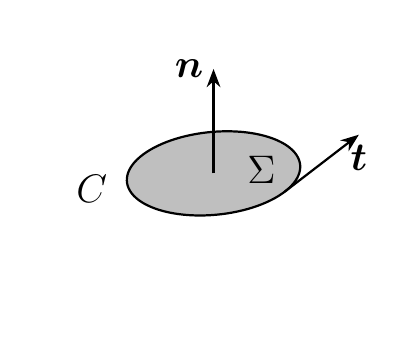
\begin{tikzpicture}[font=\Large]
  \begin{axis}[
    view={120}{40},
    hide axis,
    scale=2,
    xmin=-2, xmax=2, ymin=-2, ymax=2, zmin=0, zmax=4,
    enlarge y limits=0.1,
  ]

    \addplot3[black, thick, fill=black!25, variable=\t, domain=0:360, samples=100, samples y=1] ( {0.5*cos(t)}, {0.5*sin(t)}, {2.5});
    \node[left] at (axis cs: 0.4,-0.4,2.5) {$C$};
    \node[right] at (axis cs: -0.1,0.1,2.5) {$\Sigma$};
    \draw[-Stealth, thick, black] (axis cs:0,0,2.5) -- (axis cs: 0,0,3.5) node[left] {$\boldsymbol{n}$};
    \draw[-Stealth, thick, black] (axis cs:0,0.5,2.5) -- (axis cs: -0.75,0.5,2.5) node[below] {$\boldsymbol{t}$};
  \end{axis}

  \draw[white] (4.5, 4.5) rectangle (9,8.2);


\end{tikzpicture}
\end{document}